\section{Список смежности Ia}
\subsection{Условие задания}
\textbf{Вариант 5:} Для каждой вершины орграфа вывести её степень.

\subsection{Примеры исходного кода}
Для нахождения и вывода степени каждой вершины был создан вспомогательный
компонент \mitext{VertexPowers}, который находит степени вершин и выводит
их в виде таблицы:
\begin{minted}{jsx}
function VertexPowers() {
  const adjList = graph.current!.getAdjacencyList()
  const powers = new Map()

  for (const [k, v] of adjList) {
    powers.set(k, v.length)
    for (const [otherK, otherV] of adjList) {
      if (k === otherK) continue

      if (otherV.find(value => value[0] === k)) {
        powers.set(k, powers.get(k) + 1)
      }
    }
  }

  return (
    <TableBody>
      {graph.current!.getAdjacencyList().map(item => {
        return (
          <TableRow key={item[0]}>
            <TableCell align='right'>{item[0]}</TableCell>
            <TableCell align='left'>{powers.get(item[0])}</TableCell>
          </TableRow>
        )
      })
      }
    </TableBody>
  )
}
\end{minted}

\subsection{Краткое описание алгоритма}
Для каждой вершины подсчитывается степень исхода и степень захода,
а затем суммируются.

\subsection{Примеры входных и выходных данных}
\subsubsection{Входные данные}
\begin{figure}[H]
  \begin{minipage}{0.5\textwidth}
    \centering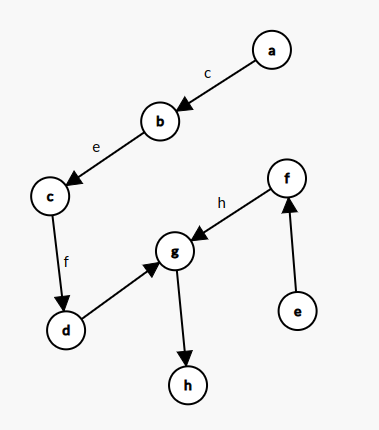
\includegraphics[width=\linewidth]{figs/task-2/graph-1.png}
  \end{minipage}
  \begin{minipage}{0.5\textwidth}
    \centering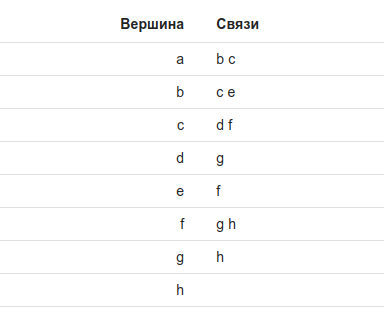
\includegraphics[width=\linewidth]{figs/task-2/adj-1.png}
  \end{minipage}
  \caption{Ориентированный граф}
\end{figure}

\begin{minted}{js}
{
  "weighted": false,
  "oriented": true,
  "adj": {
    "a": {
      "b": 0,
      "c": 0
    },
    "b": {
      "c": 0,
      "e": 0
    },
    "c": {
      "d": 0,
      "f": 0
    },
    "d": {
      "g": 0
    },
    "e": {
      "f": 0
    },
    "f": {
      "g": 0,
      "h": 0
    },
    "g": {
      "h": 0
    },
    "h": {}
  }
}
\end{minted}

\subsubsection{Выходные данные}
\begin{figure}[H]
  \centering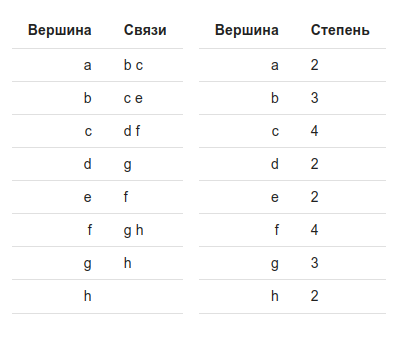
\includegraphics[width=0.5\textwidth]{figs/task-2/res-1.png}
  \caption{Результат работы}
\end{figure}